\documentclass{article}
\usepackage{amsmath}
\usepackage[utf8]{inputenc}
\usepackage{listings}
\usepackage{graphicx}

\graphicspath{ {../results/} }

\lstset{
	basicstyle=\footnotesize,
	numbers=left,
	tabsize=3,
	title=\lstname,
	breaklines=true
}

\addtolength{\oddsidemargin}{-.875in}
\addtolength{\evensidemargin}{-.875in}
\addtolength{\textwidth}{1.75in}

\addtolength{\topmargin}{-.875in}
\addtolength{\textheight}{1.75in}

\title{Lernverfahren autonomer Roboter - Übung 8}
\author{G10\\ Andre Osse\\ Waldemar Stockmann\\ Markus Strehling\\ Tobias Hahn}	
	
\begin{document}
\maketitle
\newpage
\section{Decision Tree}

\subsection{Continous data}
Bei andauernden Datenströmen kann man einen Entscheidungsbaum schlecht lernen, da für die Entscheidung, welches Attribut man für die nächste Entscheidung nimmt, statistische Daten über die Verteilung der Labels anfallen, welche nur mit annähernd kompletten Daten herausgefunden werden können.

\subsection{Same path twice}
In dem selben Pfad wird das gleiche Attribut nie zweimal getestet, da davon ausgegangen wird dass das Ergebnis dieser Abfrage immer eindeutig ist, d.h. die Ausprägungen des Attributs sind immer eindeutig und bleiben es auch. Dann macht es nicht Sinn, das gleiche Attribut nocheinmal abzufragen, da ja die Subbäume die Ausprägungen des Attributs unter sich aufteilen. Sinn machen würde dies dann, wenn das Attribut nicht eindeutig ist, also einmal den einen Wert und dann wieder einen anderen annehmen, oder gleich mehrere Ausprägungen aufeinmal annehmen kann. In diesem Fall macht zweimal nachfragen Sinn, da unterschiedliche Ergebnisse entstehen können, also sich der Knoten wieder in Subbäume aufspalten würde.

\subsection{Information gain}
Der Gain einer Partitionierung ist gegeben durch die Formel
\paragraph{}
\[
	Gain(X,T) = Info(T) - Info(X,T)
\]
\paragraph{}
Um also zu zeigen dass der Gain von der Partitionierung 0 ist, muss gezeigt werden dass $Info(T) = Info(X,T)$.
Dafür ist es hilfreich, sich deren Definitionen zu vergegenwärtigen. Die verwendeten Zeichen sind:
\paragraph{}
\begin{itemize}
	\item n = Anzahl der negativen Beispiele
	\item p = Anzahl der positiven Beispiele
	\item $|T_i|$ = Anzahl der Elemente in Partition i
	\item |T| = Gesamtanzahl der Elemente
	\item $n_i$ = Anzahl der negativen Beispiele in Partition i
	\item $p_i$ = Anzahl der positiven Beispiele in Partition i
\end{itemize}
\paragraph{}
\begin{align*}
	Info(T) &= I(\frac{p}{p+n},\frac{n}{p+n}) = -(\frac{p}{p+n} * log_2(\frac{p}{p+n}) + \frac{n}{p+n} * log_2(\frac{n}{p+n})) \\
	Info(X,T) &= \sum_i \frac{|T_i|}{|T|} I(\frac{p_i}{p_i+n_i},\frac{n_i}{p_i+n_i})
\end{align*}

Wir wissen, dass $\frac{p_i}{p_i+n_i}$ für alle Partitionen gleich ist. Nun müssen wir noch zeigen dass daraus auch folgt dass $\frac{n_i}{p_i+n_i}$ für alle Partitionen gleich ist, dass hätten wir gezeigt dass wir uns das gewichtete Mitteln sparen können, da das gewichtete Mitteln von immergleichen Zahlen immer die gleiche Zahl ergibt. Dies ist jedoch einfach zu zeigen, da $\frac{n_i}{p_i+n_i} = 1 - \frac{p_i}{p_i+n_i}$, d.h. wenn das eine für alle gleich ist ist das andere Verhältnis auch für beide gleich. Damit kann man die zweite Gleichung vereinfachen zu: 
\paragraph{}
\[
	Info(X,T) = I(\frac{p_i}{p_i+n_i},\frac{n_i}{p_i+n_i})
\]
\paragraph{}
Diese vereinfachte Form sieht nun schon fast so aus wie der Informationsgehalt von Info(T), nur dass statt der Gesamtanzahl von n und p jeweils die Anzahlen in einer der Partitionen stehen. Da wir aber gezeigt haben dass beide Verhältnisse in allen Partitionen gleich sind, so folgt daraus dass das Verhältnis auch in der Summe der Partitionen das gleiche ist. D.h. Info(T) = Info(X,T), und damit Gain = 0.

\subsection{Decision tree learning}
\subsubsection{Code}
\lstinputlisting{../code/decisiontree.py}
\subsubsection{Plot}
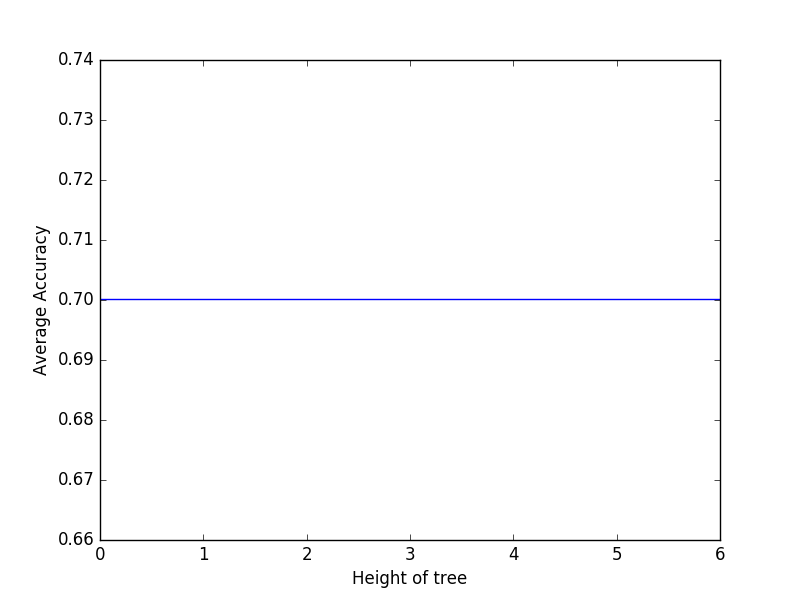
\includegraphics[width=\textwidth]{accuracies.png}
\subsubsection{Visualisation}
\begin{lstlisting}
[safety](None)
|[buying](high)
|[buying](med)
|[buying](low)
||=unacc
||=unacc
||=unacc
||=unacc
||=unacc
||=unacc
||=unacc
||=unacc
||=unacc
||=unacc
||=unacc
||=unacc
\end{lstlisting}

\section{Support Vector Machines}
\subsection{Unequal Classes}
Wenn die Klassenverteilung sehr ungleich ist, dann tritt bei SVM folgendes Problem auf: Da wir den Abstand der Datenpunkte zur Hyperebene maximieren, kann es Sinn machen die Trennlinie möglichst weit von den Punkten der größeren Klasse wegzuschieben, auch wenn dabei die Trennschärfe verloren geht, da der Abstand der zu den Punkten der großen Menge gewonnen wird größer ist als der der verloren geht dadurch dass der Abstand zu den kleineren Punkten verloren geht. Damit würde SVM nicht mehr richtig klassifizeren, obwohl das Maximierungsziel erreicht wurde.

\subsection{Workings}
Das Maximisierungsproblem von SVM besteht darin den Abstand der Datenpunkte von der Hyperebene zu maximieren. Dafür wird eine entsprechende Fehlerfunktion gewählt, welche nicht einfach nur die richtige Klassifizerung des Datenpunkts angibt, sondern wieviel Abstand zwischen der Trennlinie und dem Datenpunkt besteht. Der wichtigste Tuningfaktor ist dabei C, also der Faktor der angibt wie wichtig es relativ ist, den Fehler zu minimieren, anstatt die Regularisierungskomponente zu maximieren. Ist dieser Faktor zu gering gewählt, so achtet der Algorithmus eher darauf die Gewichte der Linie minimal zu halten, anstatt richtig zu klassifizieren. Ist er zu groß gewählt, so maximiert der Algorithmus die Klassifizerung, wodurch Outlier die Hyperebene stark beeinflussen und den Abstand zu den Datenpunkten verringert.

\subsection{Kerneltrick}
Normalerweise schafft es SVM nur, Datenpunkte linear zu trennen. Dies kann jedoch ein Problem sein, wenn Datenpunkte gar nicht linear getrennt sind sondern z.B. polynomial. Hier kann man abhilfe schaffen, indem man die Datenpunkte in neue Datenpunkte mappt, mithilfe eines Kernels. Dieser gibt uns an wie ein Datenpunkt gemappt wird, z.B. x auf $x^2$. Nun wird dieser Abstand maximiert, wodurch sich Trennlinien ergeben können die nicht linear sind. Prinzipiell kann es immer angewandt werden wenn man einen Kernel hat und der Kernel gewisse Bedingungen erfüllt.

\subsection{Decision Boundary}
Die Decision Boundary verändert sich natürlich, wenn der Kernel gewechselt wird. Dies liegt daran dass nun die Fehlerfunktion nicht mehr auf die Datenpunkte, sondern auf die gemappten Datenpunkte angewandt wird, d.h. der Abstand zwischen zwei Punkten kann sich gewaltig verändern, wodurch sich auch die Decision Boundary verändert.

\end{document}
